\subsection{理论依据}
$E(Z)=0,var(Z)=I_p,$则有$S_{Y|Z}$是$\Sigma_{ZZY}$的不变子空间。

又有$\Sigma_{ZY} \in S_{Y|Z}$,由此可得$\Sigma_{ZY},\Sigma_{ZZY}\Sigma_{ZY},\Sigma_{ZZY}^2\Sigma_{ZY},\dots,\Sigma_{ZZY}^{p-1}\Sigma_{ZY} \in S_{Y|Z}$
\subsection{算法流程}
\begin{enumerate}
    \item 将$X_1,\dots,X_n$标准化为$Z_1,\dots,Z_n$
    \item 计算$\hat{\Sigma}_{ZY}=Cov_n(Z,Y),\hat{\Sigma}_{ZZY}=E_n(ZZ^TY)$
    \item 计算$p\times p$矩阵$\hat{M}=(\hat{\Sigma}_{ZY},\hat{\Sigma}_{ZZY}\hat{\Sigma}_{ZY},\hat{\Sigma}_{ZZY}^2\hat{\Sigma}_{ZY},\dots,\hat{\Sigma}_{ZZY}^{p-1}\hat{\Sigma}_{ZY})$
并记$\hat{\Lambda}=\hat{M}\hat{M}^T$
    \item 计算$\hat{\Lambda }$的前$q$个特征向量$u_1,\dots,u_q$,并令$v_k=\hat{\Sigma}_{XX}^{-1/2}u_k,k=1,\dots,q$
    \item 则估计量为$\{v_k^T[X_i-E_n(X)]:i=1,\dots,n\},\quad k=1,\dots,q$
\end{enumerate}
\subsection{线性回归模型}

设置降维维度为二维,即按$y=\beta_1^Tx+\beta_2^Tx+\varepsilon$,生成样本y。其中$\beta_1$是参数矩阵$\beta$的第一列向量,同理$\beta_2$,而$\varepsilon$服从均值为0,方差0.1的正态分布。设定样本量为1000,降维维数由$10-20$,判断其降维效果.
\begin{figure}[H]
    \centering
    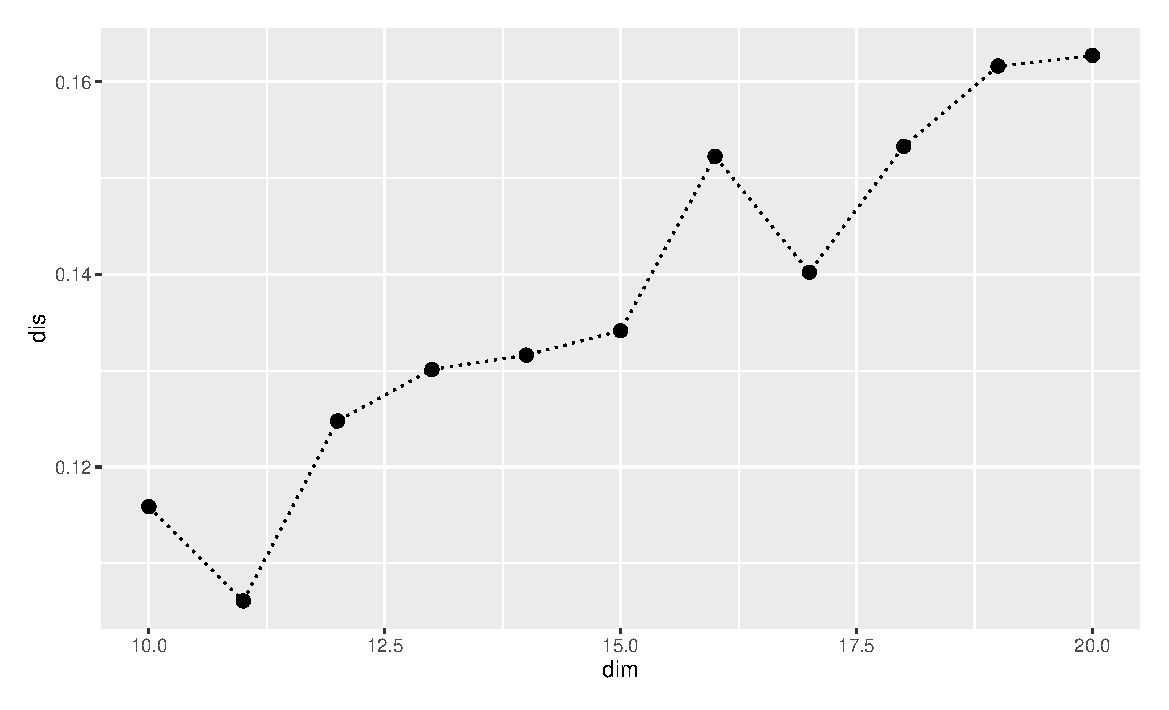
\includegraphics[width=0.8\textwidth]{image/norm_iht.eps}
    \caption{线性回归下维度对降维效果的影响}
\end{figure}




\subsection{对数似然回归}

按$y = \frac{1}{1+\exp{(-\beta^Tx)}}+ \varepsilon$关系生成样本$y$,$\varepsilon \sim N(0,0.1)$,设定样本量为1000,降维维数由$10-20$,判断其降维效果.
\begin{figure}[H]
    \centering
    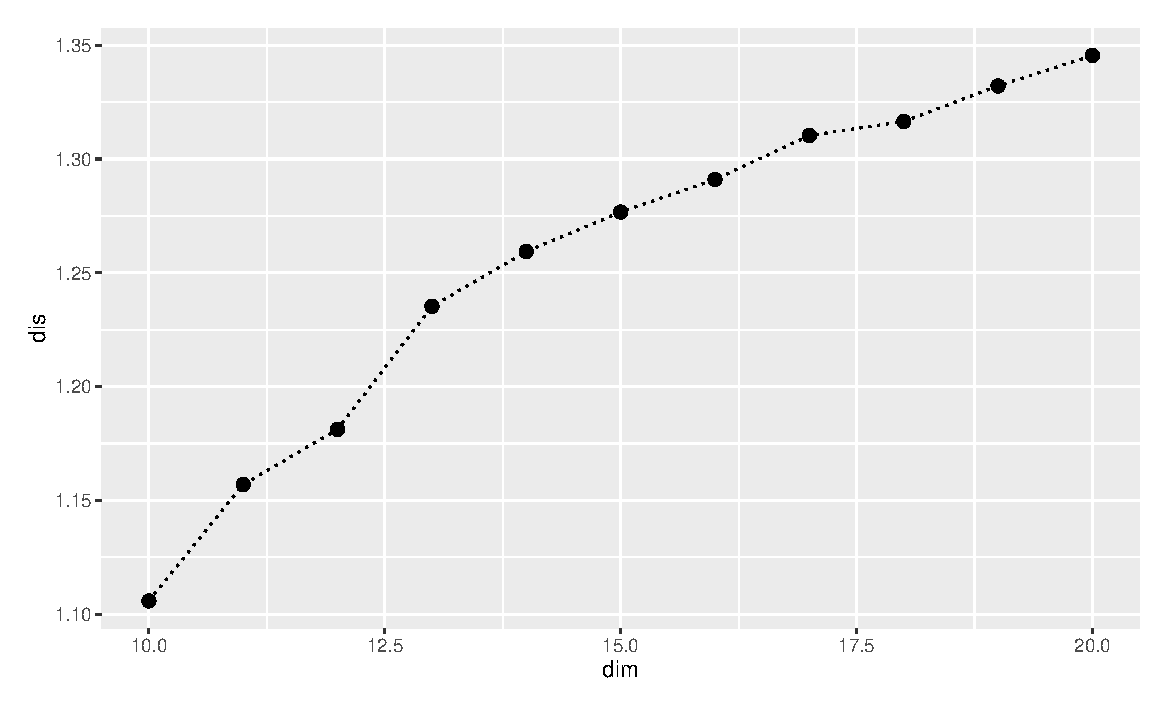
\includegraphics[width=0.8\textwidth]{image/logit_save.eps}
    \caption{logistic回归下维度对降维效果的影响}
\end{figure}


\subsection{$\cos$与$\sin$函数关系}

按$y=\sin(2\beta_1^Tx)+\cos(\beta_2^Tx)+\varepsilon$,生成样本y。其中$\beta_1$是参数矩阵$\beta$的第一列向量,同理$\beta_2$,而$\varepsilon$服从均值为0,方差0.1的正态分布。对于$\sin$函数关系,我们按$y=\sin(2\beta_1^Tx)+\sin(\beta_2^Tx)+\varepsilon$,生成样本y.
\begin{figure}[H]
    \centering
    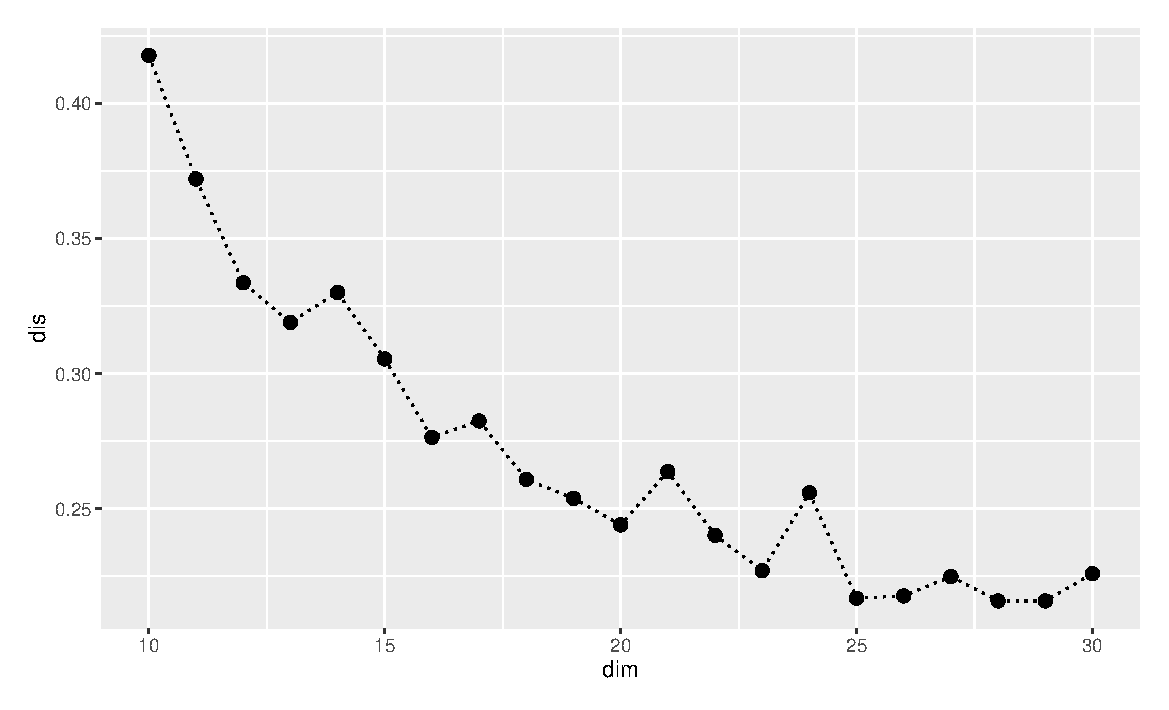
\includegraphics[width=0.8\textwidth]{image/cos_sin_iht.eps}
    \caption{三角函数生成的数据下维度对降维效果的影响}
\end{figure}
可以看出在降维子空间在25维之后降维效果有下降的趋势,由于计算时间过长,本次试验没有进行更高维度的判断.


\subsection{三角函数在IHT与PHD下降维效果的对比}
按$y=\cos(2\beta_1^Tx)+\sin(\beta_2^Tx)+\varepsilon$,生成样本y. 分别使用PHD方法与IHT方法进行降维.
\begin{equation}       %开始数学环境
    \beta_{phd}= \left(                 %左括号
       \begin{array}{cc}   %该矩阵一共3列,每一列都居中放置
          0.948449657  &  0.01971554 \\
         -0.047997173  &  0.29983925 \\
          0.034641505  & -0.19857183 \\
          0.008065384  &  0.69594286 \\
         -0.073057556  & -0.31804108 \\
          0.027100694  &  0.13619042 \\
         -0.130396457  & -0.26034245 \\
          0.171602330  & -0.11436164 \\
          0.068274073  & -0.33846860 \\
          0.081761191  & -0.21252464 \\
       \end{array}
     \right)                 %右括号
 \end{equation}


 \begin{equation}       %开始数学环境
    \beta_{iht}= \left(                 %左括号
       \begin{array}{cc}   %该矩阵一共3列,每一列都居中放置
          0.976733646  & -0.0647860186 \\
         -0.019360699  & -0.9058644433 \\
          0.015809941  &  0.4508445520 \\
          0.006769810  &  0.1351203693 \\
         -0.016888058  & -0.0002618049 \\
          0.007019351  & -0.0178304939 \\
         -0.010093698  &  0.0408656636 \\
          0.008968595  & -0.0299744106 \\
          0.017278169  &  0.0001168891 \\
         -0.003163035  & -0.0225223252 \\
       \end{array}
     \right)                 %右括号
 \end{equation}


可以看出IHT方法处理此类函数关系时的降维效果要明显由于PHD方法,即虽然在$H_1$方向下的降维效果接近真实值,但是在$H_2$方向下降维效果PHD要劣于IHT.